\documentclass{article}
\usepackage{enumitem}
\usepackage{indentfirst}
\usepackage{listings}
\usepackage{tikz}
\usepackage{caption}
\usepackage[romanian]{babel}
\usepackage{amsmath}
\usepackage{amsfonts}
\usepackage[a4paper,portrait,margin=1in]{geometry}
\usepackage{wrapfig}
\usetikzlibrary{arrows.meta}
\pagenumbering{gobble}

\renewcommand\thesection{\arabic{section}.}
\renewcommand\thesubsection{\thesection\arabic{subsection}.}
\renewcommand\labelitemii{$\circ$}
\newcommand{\qu}[1]{„\emph{#1}”}
\DeclareMathOperator{\tg}{tg}
\DeclareMathOperator{\ctg}{ctg}
\DeclareMathOperator{\arctg}{arctg}
\DeclareMathOperator{\arcctg}{arcctg}
\DeclareMathOperator{\dist}{dist}

\title{Geometrie și trigonometrie}
\author{}
\date{}
\begin{document}
\maketitle
\section*{Formule trigonometrice}
\begin{align*}
    \begin{split}
        \sin(-x) &= -\sin x \\
        \cos(-x) &= \cos x
    \end{split} &
    \begin{split}
        \sin\left(\frac{\pi}{2} - x\right) &= \cos x \\
        \cos\left(\frac{\pi}{2} - x\right) &= \sin x
    \end{split} &
    \begin{split}
        \sin(\pi - x) &= \sin x \\
        \cos(\pi - x) &= -\cos x
    \end{split} &
    \textbf{fct}(\frac{k\pi}{2} \pm x) = \left\{\begin{array}{ll}
        \pm\ \textbf{fct} x & k\ \text{e par} \\
        \pm\ \textbf{cofct} x & k\ \text{e impar}
    \end{array}\right.
\end{align*}
\begin{align*}
    \sin(x\pm y) &= \sin x \cos y \pm \sin y \cos x &
    \sin(2x) &= 2\sin x \cos x &
    \sin(3x) &= 3\sin x - 4\sin^3 x \\
    \cos(x\pm y) &= \cos x \cos y \mp \sin x \sin y &
    \cos(2x) &= \cos^2 x - \sin^2 x &
    \cos(3x) &= 4\cos^3 x - 3\cos x
\end{align*}
\begin{align*}
    \tg(x\pm y) &= \frac{\tg x \pm \tg y}{1 \mp \tg x \tg y} &
    \cos^2 x &= \frac{1 + \cos(2x)}{2} \\
    \tg(2x) &= \frac{2 \tg x}{1 - \tg^2 x} &
    \sin^2 x &= \frac{1 - \cos(2x)}{2}
\end{align*}
\begin{align*}
    \sin x \pm \sin y &= 2 \sin \frac{x \pm y}{2} \cos \frac{x \mp y}{2} &
    \sin x \cos y &= \frac{\sin(x-y)+\sin(x+y)}{2} \\
    \cos x + \cos y &= 2 \cos \frac{x+y}{2} \cos \frac{x-y}{2} &
    \cos x \cos y &= \frac{\cos(x-y)+\cos(x+y)}{2} \\
    \cos x - \cos y &= -2 \sin \frac{x+y}{2} \sin \frac{x-y}{2} &
    \sin x \sin y &= \frac{\cos(x-y) - \cos(x+y)}{2}
\end{align*}
\begin{align*}
    \tg x \pm \tg y &= \frac{\sin(x\pm y)}{\cos x \cos y} &
    1 + \tg^2 x &= \frac{1}{\cos^2 x} = (\tg x)'
\end{align*}
\begin{align*}
    \sin x &= \frac{2\tg \frac{x}{2}}{1 + \tg^2 \frac{x}{2}} &
    \sin x &= \pm \frac{\tg x}{\sqrt{1+\tg^2 x}} \\
    \cos x &= \frac{1 - \tg^2 \frac{x}{2}}{1 + \tg^2 \frac{x}{2}} &
    \cos x &= \pm \frac{1}{\sqrt{1+\tg^2 x}}
\end{align*}
\begin{align*}
    \arcsin x + \arccos x &= \frac{\pi}{2}\quad \forall x \in [-1, 1] &
    \arctg x + \arcctg x &= \frac{\pi}{2}\quad \forall x \in \mathbb{R}
\end{align*}
\begin{align*}
    \sin(\arccos x) &= \sqrt{1-x^2} &
    \sin(\arctg x) &= \frac{x}{\sqrt{1+x^2}} \\
    \cos(\arccos x) &= \sqrt{1-x^2} &
    \cos(\arctg x) &= \frac{1}{\sqrt{1+x^2}}
\end{align*}
\section*{Ecuații trigonometrice}
\begin{minipage}{\textwidth}
\textbf{Ecuații trigonometrice elementare}:
\begin{align*}
\sin x = a &\implies x = (-1)^k \arcsin a + k\pi \\
\cos x = a &\implies x = \pm \arccos a + 2k\pi \\
\tg x = a &\implies x = \arctg a + k\pi
\end{align*}
pentru $k \in \mathbb{Z}$.
\end{minipage}

Pentru $a, b, c$ date avem \textbf{ecuații trigonometrice liniare} de forma:
\begin{equation*}
    a\sin x + b\cos x = c
\end{equation*}
care se rezolvă astfel:
\begin{enumerate}
    \item Dacă $(a, b) \in \{(\pm 1, \pm 1), (\pm 1, \pm \sqrt{3}), (\pm \sqrt{3}, 1)\}$, atunci se folosește metoda unghiului auxiliar.
    \item Altfel, verificăm dacă $x=\pi$ este sau nu soluție.
    \begin{itemize}
        \item Dacă da, atunci $x = \pi + 2k\pi$ sunt soluții, pentru $k \in \mathbb{Z}$.
    \end{itemize}
    \item După aceea, putem folosi formulele:
    \begin{align*}
        \sin x &= \frac{2\tg \frac{x}{2}}{1 + \tg^2 \frac{x}{2}} &
        \cos x &= \frac{1 - \tg^2 \frac{x}{2}}{1 + \tg^2 \frac{x}{2}}
    \end{align*}
    Notăm $\tg \frac{x}{2} = t$, și avem o ecuație de gradul II în $t$ pe care o rezolvăm. Apoi rezolvăm $\tg \frac{x}{2} = t$.
\end{enumerate}
\section*{Formule în triunghi}
\begin{tikzpicture}
    \coordinate [label=above:$A$] (A) at (2, 4);
    \coordinate [label=left:$B$] (B) at (0, 0);
    \coordinate [label=right:$C$] (C) at (6, 0);
    \draw (A) -- node[left] {$c$} (B) -- node[below] {$a$} (C) -- node[above] {$b$} (A);
\end{tikzpicture}
\begin{itemize}
    \item \textbf{Semiperimetru}: $p = \frac{a+b+c}{2}$
    \item \textbf{Suprafață}: $S = \frac{\textbf{bază}\cdot\textbf{înălțime}}{2} = \frac{a b \sin C}{2} = \sqrt{p(p-a)(p-b)(p-c)}$
    \item \textbf{Raza cercului înscris în triunghi}: $r = \frac{S}{p}$
    \item \textbf{Raza cercului circumscris triunghiului}: $R = \frac{abc}{4S}$
    \item \textbf{Teorema sinusurilor}: $\frac{a}{\sin A} = \frac{b}{\sin B} = \frac{c}{\sin C} = 2R$
    \item \textbf{Teorema cosinusului}: $a^2 = b^2 + c^2 - 2bc\cos A$
    \item $\sin \frac{A}{2} = \sqrt{\frac{(p-b)(p-c)}{bc}}$
    \item $\cos \frac{A}{2} = \sqrt{\frac{(p)(p-a)}{bc}}$
\end{itemize}
\section*{Vectori}
Un vector $\overrightarrow{AB}$ are:
\begin{itemize}
    \item \textbf{Direcție}: dreapta $AB$, sau orice paralelă la aceasta.
    \item \textbf{Sens}: de la $A$ la $B$.
    \item \textbf{Mărime}: lungimea segmentului $[AB]$. Este, de asemena, \textbf{modulul} vectorului.
\end{itemize}

Atunci când vectorul nu este cuplat într-un sistem de axe de coordonate, vorbim despre un \textbf{vector liber}, altfel vorbim despre un \textbf{vector legat}.
\subsection*{Vectori liberi}
Următoarele aspecte se pot aplica atât vectorilor liberi, cât și celor legați:
\begin{itemize}
    \item \textbf{Vectori egali}: $\overrightarrow{AB} = \overrightarrow{CD}$ dacă $AB \parallel CD$, $[AB] \equiv [CD]$ și dacă au același sens.
    \item \textbf{Adunarea vectoilor}:
    \begin{itemize}
        \item[] \begin{tikzpicture}
            \coordinate [label=left:$A$] (A) at (2, 4);
            \coordinate [label=left:$B$] (B) at (0, 0);
            \coordinate [label=right:$C$] (C) at (6, 0);
            \coordinate [label=right:$D$] (D) at (8, 4);
            \fill (A) circle[radius=2pt];
            \draw [-{Stealth[scale=1.5]}] (A) -- (B);
            \draw [-{Stealth[scale=2.25]}] (A) -- (C);
            \draw [-{Stealth[scale=1.5]}] (A) -- (D);
            \draw (B) -- (C);
            \draw (D) -- (C);
        \end{tikzpicture}
        \item \textbf{Regula paralelogramului}: În $ABCD$ paralelogram, $\overrightarrow{AB}+\overrightarrow{AD}=\overrightarrow{AC}$.\item[] \begin{tikzpicture}
            \coordinate [label=right:$A$] (A) at (4, 4);
            \coordinate [label=left:$B$] (B) at (0, 0);
            \coordinate [label=right:$C$] (C) at (5, 0);
            \fill (A) circle[radius=2pt];
            \draw [-{Stealth[scale=1.5]}] (A) -- (B);
            \draw [-{Stealth[scale=2.25]}] (A) -- (C);
            \draw [-{Stealth[scale=1.5]}] (B) -- (C);
        \end{tikzpicture}
        \item \textbf{Regula triunghiului}: $\overrightarrow{AB}+\overrightarrow{BC}=\overrightarrow{AC}$.
        \item Pentru 2 vectori oarecare $\overrightarrow{AB}$, $\overrightarrow{CD}$, se alege un punct $O$, apoi avem $\overrightarrow{AB} = \overrightarrow{OM}$, $\overrightarrow{CD} = \overrightarrow{MN}$, iar $\overrightarrow{AB}+\overrightarrow{BC}=\overrightarrow{ON}$.
    \end{itemize}
    \item \textbf{Înmulțirea cu un număr}: $k\cdot \overrightarrow{AB}$. Rezultă un vector cu $|k\cdot \overrightarrow{AB}| = |k|\cdot|\overrightarrow{AB}|$, direcția păstrată, iar sensul inversat dacă $k<0$.
    \item \textbf{Produsul scalar}: $\overrightarrow{AB}\times\overrightarrow{CD} = |\overrightarrow{AB}|\cdot|\overrightarrow{CD}|\cdot\cos(\widehat{\overrightarrow{AB}, \overrightarrow{CD}})$.
    \begin{itemize}
        \item Grijă la semnul cosinusului! Unghiul se măsoară ducând în același punct originile vectorilor. Dacă cei doi vectori par să \textit{meargă în sensuri opuse}, semnul este de regulă minus!
    \end{itemize}
    \item În $\triangle ABC$, cu $P \in (BC)$, $\frac{BP}{PC} = k$ avem $\overrightarrow{AP}=\frac{\overrightarrow{AB}+k\overrightarrow{AC}}{1+k}$.
    \begin{itemize}
        \item În $\triangle ABC$, cu $P$ mijlocul lui $[BC]$, avem $\overrightarrow{AP}=\frac{\overrightarrow{AB}+\overrightarrow{AC}}{2}$.
    \end{itemize}
    \item $A, B, C$ sunt \textbf{coliniare} $\iff \exists k \in \mathbb{R}$ a.î. $\overrightarrow{AB} = k \cdot \overrightarrow{BC}$.
    \begin{itemize}
        \item $AB \parallel CD$ sau $AB = CD$ (dreptele sunt identice) $\iff \exists k \in \mathbb{R}$ a.î. $\overrightarrow{AB} = k \cdot \overrightarrow{CD}$.
    \end{itemize}
    \item $ABCD$ este \textbf{paralelogram} $\iff \overrightarrow{AB}=\overrightarrow{DC} \iff \exists O \in \textit{plan}$ a.î. $\overrightarrow{OA}+\overrightarrow{OC}=\overrightarrow{OB}+\overrightarrow{OD}$.
    \item Dacă $ABCD$ este paralelogram cu $|\overrightarrow{AB}+\overrightarrow{AD}|=|\overrightarrow{AB}-\overrightarrow{AD}|$, atunci $ABCD$ este \textbf{dreptunghi}.
    \item $G$ este \textbf{centru de greutate} în $\triangle ABC$ dacă, pentru un punct $O$,\quad  $\overrightarrow{OG}=\frac{\overrightarrow{OA}+\overrightarrow{OB}+\overrightarrow{OC}}{3}$.
    \item \textbf{Inegalitate triunghiulară}: $|\overrightarrow{AB}+\overrightarrow{AC}| \leq |\overrightarrow{AB}|+|\overrightarrow{AC}|$.
\end{itemize}
\subsection*{Vectori legați}
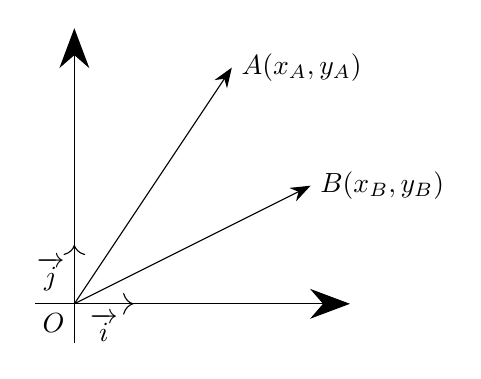
\begin{tikzpicture}
    \coordinate [label=right:{$A (x_A, y_A)$}] (A) at (2, 3);
    \coordinate [label=right:{$B (x_B, y_B)$}] (B) at (3, 1.5);
    \coordinate [label=below left:$O$] (O) at (0, 0);
    \coordinate (i) at (0.75, 0);
    \coordinate (j) at (0, 0.75);
    \draw [-{Stealth[scale=3]}] (-0.5, 0) -- (3.5, 0);
    \draw [-{Stealth[scale=3]}] (0, -0.5) -- (0, 3.5);
    \draw [-{Stealth[scale=1.5]}] (O) -- (A);
    \draw [-{Stealth[scale=1.5]}] (O) -- (B);
    \draw [-{To[scale=1.5]}] (O) -- node[below] {$\overrightarrow{i}$} (i);
    \draw [-{To[scale=1.5]}] (O) -- node[left] {$\overrightarrow{j}$} (j);
\end{tikzpicture}
\begin{itemize}
    \item \textbf{Versori}: $\overrightarrow{i}$ (abscise), $\overrightarrow{j}$ (ordonate). $|\overrightarrow{i}|=|\overrightarrow{j}|=1$.
    \item \textbf{Vector de poziție}: $\overrightarrow{r_A} = \overrightarrow{OA} = x_A \overrightarrow{i} + y_A \overrightarrow{j}$. Avem $|\overrightarrow{OA}|=\sqrt{{x_A}^2+{y_A}^2}$.
    \item $\overrightarrow{OA} + \overrightarrow{OB} = (x_A+x_B)\overrightarrow{i} + (y_A+y_B)\overrightarrow{j}$.
    \item $\overrightarrow{AB} = \overrightarrow{OA} - \overrightarrow{OB} = (x_A-x_B)\overrightarrow{i} + (y_A-y_B)\overrightarrow{j}$.
\end{itemize}
Avem $\overrightarrow{u}=a\overrightarrow{i}+b\overrightarrow{j}$, $\overrightarrow{v}=p\overrightarrow{i}+q\overrightarrow{j}$ vectori legați:
\begin{itemize}
    \item \textbf{Produsul scalar}: $\overrightarrow{u}\times\overrightarrow{v} = ap + bq$.
    \item $\overrightarrow{u}$ și $\overrightarrow{v}$ sunt \textbf{coliniare} $\iff \frac{a}{p} = \frac{b}{q}$.
    \item $\overrightarrow{u}$ și $\overrightarrow{v}$ sunt \textbf{perpendiculare} $\iff \overrightarrow{u}\times\overrightarrow{v} = ap + bq = 0$.
    \item \textbf{Inegalitatea Cauchy-Buniakovski-Schwartz pentru vectori}: $\overrightarrow{u}\times\overrightarrow{v} \leq |\overrightarrow{u}|\cdot|\overrightarrow{v}|$.
\end{itemize}
\section*{Geometrie analitică}
\subsection*{Puncte}
Pentru $A(x_A, y_A)$, $B(x_B, y_B)$ avem:
\begin{itemize}
    \item \textbf{Lungimea segmentului} $AB = \sqrt{(x_A-x_B)^2+(y_A-y_B)^2}$.
    \item \textbf{Mijlocul segmentului}: $M(\frac{x_A+x_B}{2}, \frac{y_A+y_B}{2})$.
\end{itemize}
\subsection*{Drepte}
\begin{itemize}
    \item \textbf{Ecuația dreptei} $d$: $ax + by + c = 0$, unde $a, b, c \in \mathbb{R}$, $a^2+b^2 \neq 0$ ($a$ și $b$ să nu fie simultan $0$).
    \begin{itemize}
        \item $A \in d \iff ax_A + by_A +c = 0$.
        \item \textbf{Ecuația carteziană}: $y = mx + n$, unde $m$ este \textbf{panta}, sau $\tg(\widehat{Ox, d})$.
    \end{itemize}
    \item \textbf{Ecuația dreptei ce trece prin 2 puncte} $A$, $B$: $AB: \frac{y-y_A}{y-y_B}=\frac{x-x_A}{x-x_B}$, sau $\left|\begin{matrix}
        x & y & 1 \\
        x_A & y_A & 1 \\
        x_b & y_B & 1
    \end{matrix}\right| = 0$.
    \item \textbf{Ecuația dreptei ce trece prin} $A$, \textbf{cu pantă} $m$ \textbf{dată}: $y-y_A = m(x-x_A)$.
    \item \textbf{Ecuația tangentei în $(a, f(a))$ la graficul lui $f$ dat}: $y-f(a)=f'(a)(x-a)$.
    \item \textbf{Distanța de la punctul $A$ la dreapta $d$}: $\dist(A, d)=\frac{|ax_A+by_A+c|}{\sqrt{a^2+b^2}}$.
\end{itemize}
Pentru 2 drepte $d_1 : ax+by+c=0$, $d_2 : px+qy+r=0$ avem:
\begin{itemize}
    \item \textbf{Paralelitate}: $d_1 \parallel d_2 \iff \frac{a}{p} = \frac{b}{q} = \frac{c}{r}$.
    \item \textbf{Perpendicularitate}: $d_1 \perp d_2 \iff ms=-1$ (produsul pantelor e egal cu $-1$).
    \item \textbf{Punctul de intersecție a dreptelor}: are coordonatele date de soluția sistemului de ecuații determinat de ecuațiile dreptelor.
\end{itemize}
\subsection*{Alte figuri geometrice}
\begin{itemize}
    \item \textbf{Aria} $\triangle ABC = \frac{1}{2}\left|\left|\begin{matrix}
        x_A & y_A & 1 \\
        x_B & y_B & 1 \\
        x_C & y_C & 1
    \end{matrix}\right|\right|$.
    \item \textbf{Ecuația cercului de rază $r$ cu centrul în origine}: $\mathcal{C}(O, r): x^2+y^2=r^2$.
\end{itemize}
\end{document}
